\documentclass[border=8pt]{standalone}
\usepackage{tikz}
\usetikzlibrary{positioning,shapes.geometric,arrows.meta,calc,backgrounds,fit}

\definecolor{enccolor}{RGB}{65,105,225}       % Royal blue - Encoder
\definecolor{deccolor}{RGB}{34,139,34}        % Forest green - Decoder
\definecolor{bottleneck}{RGB}{220,20,60}      % Crimson - Bottleneck
\definecolor{attncolor}{RGB}{255,140,0}       % Dark orange - Attention gates
\definecolor{skipcolor}{RGB}{128,128,128}     % Gray - Skip connections

\begin{document}
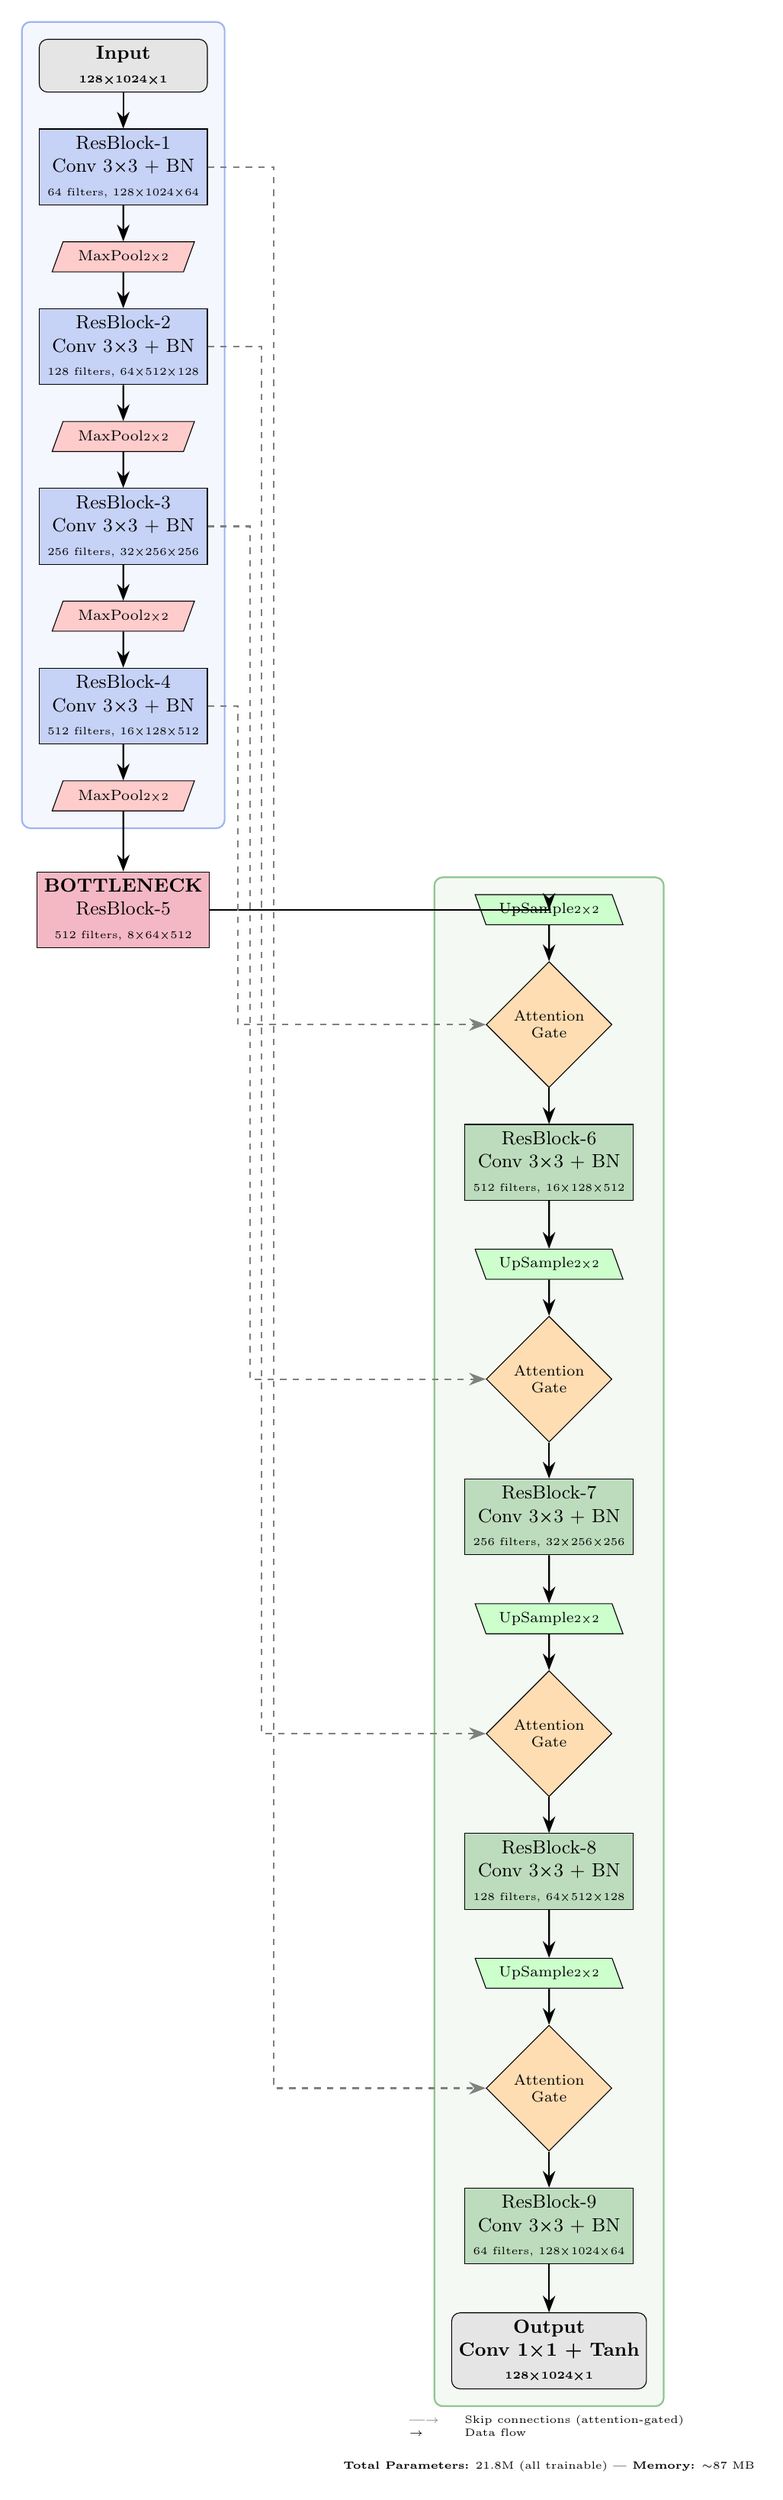
\begin{tikzpicture}[
    node distance=0.6cm,
    layer/.style={rectangle, draw, minimum width=2.8cm, minimum height=0.6cm, align=center, font=\small},
    enc/.style={layer, fill=enccolor!30},
    dec/.style={layer, fill=deccolor!30},
    bottle/.style={layer, fill=bottleneck!30, minimum height=0.8cm},
    attn/.style={diamond, draw, fill=attncolor!30, minimum width=1.8cm, minimum height=0.6cm, font=\scriptsize, align=center},
    pool/.style={trapezium, trapezium left angle=70, trapezium right angle=110, draw, fill=red!20, minimum width=1.5cm, minimum height=0.5cm, font=\scriptsize},
    upsample/.style={trapezium, trapezium left angle=110, trapezium right angle=70, draw, fill=green!20, minimum width=1.5cm, minimum height=0.5cm, font=\scriptsize},
    inout/.style={layer, fill=gray!20, rounded corners, font=\small\bfseries},
    arrow/.style={-{Stealth[scale=1.2]}, thick},
    skip/.style={-{Stealth[scale=1.2]}, thick, dashed, skipcolor},
    label/.style={font=\tiny, align=center}
]

% ===== INPUT =====
\node[inout] (input) at (0,0) {Input\\{\tiny 128×1024×1}};

% ===== ENCODER =====
\node[enc, below=of input] (enc1) {ResBlock-1\\Conv 3×3 + BN\\{\tiny 64 filters, 128×1024×64}};
\node[pool, below=of enc1] (pool1) {MaxPool\\{\tiny 2×2}};

\node[enc, below=of pool1] (enc2) {ResBlock-2\\Conv 3×3 + BN\\{\tiny 128 filters, 64×512×128}};
\node[pool, below=of enc2] (pool2) {MaxPool\\{\tiny 2×2}};

\node[enc, below=of pool2] (enc3) {ResBlock-3\\Conv 3×3 + BN\\{\tiny 256 filters, 32×256×256}};
\node[pool, below=of enc3] (pool3) {MaxPool\\{\tiny 2×2}};

\node[enc, below=of pool3] (enc4) {ResBlock-4\\Conv 3×3 + BN\\{\tiny 512 filters, 16×128×512}};
\node[pool, below=of enc4] (pool4) {MaxPool\\{\tiny 2×2}};

% ===== BOTTLENECK =====
\node[bottle, below=1cm of pool4] (bottleneck) {\textbf{BOTTLENECK}\\ResBlock-5\\{\tiny 512 filters, 8×64×512}};

% ===== DECODER (positioned to the right) =====
\node[upsample, right=4.5cm of bottleneck] (up4) {UpSample\\{\tiny 2×2}};
\node[attn, below=of up4] (att4) {Attention\\Gate};
\node[dec, below=of att4] (dec4) {ResBlock-6\\Conv 3×3 + BN\\{\tiny 512 filters, 16×128×512}};

\node[upsample, below=0.8cm of dec4] (up3) {UpSample\\{\tiny 2×2}};
\node[attn, below=of up3] (att3) {Attention\\Gate};
\node[dec, below=of att3] (dec3) {ResBlock-7\\Conv 3×3 + BN\\{\tiny 256 filters, 32×256×256}};

\node[upsample, below=0.8cm of dec3] (up2) {UpSample\\{\tiny 2×2}};
\node[attn, below=of up2] (att2) {Attention\\Gate};
\node[dec, below=of att2] (dec2) {ResBlock-8\\Conv 3×3 + BN\\{\tiny 128 filters, 64×512×128}};

\node[upsample, below=0.8cm of dec2] (up1) {UpSample\\{\tiny 2×2}};
\node[attn, below=of up1] (att1) {Attention\\Gate};
\node[dec, below=of att1] (dec1) {ResBlock-9\\Conv 3×3 + BN\\{\tiny 64 filters, 128×1024×64}};

% ===== OUTPUT =====
\node[inout, below=0.8cm of dec1] (output) {Output\\Conv 1×1 + Tanh\\{\tiny 128×1024×1}};

% ===== ARROWS - ENCODER =====
\draw[arrow] (input) -- (enc1);
\draw[arrow] (enc1) -- (pool1);
\draw[arrow] (pool1) -- (enc2);
\draw[arrow] (enc2) -- (pool2);
\draw[arrow] (pool2) -- (enc3);
\draw[arrow] (enc3) -- (pool3);
\draw[arrow] (pool3) -- (enc4);
\draw[arrow] (enc4) -- (pool4);
\draw[arrow] (pool4) -- (bottleneck);

% ===== ARROWS - DECODER =====
\draw[arrow] (bottleneck) -| (up4);
\draw[arrow] (up4) -- (att4);
\draw[arrow] (att4) -- (dec4);
\draw[arrow] (dec4) -- (up3);
\draw[arrow] (up3) -- (att3);
\draw[arrow] (att3) -- (dec3);
\draw[arrow] (dec3) -- (up2);
\draw[arrow] (up2) -- (att2);
\draw[arrow] (att2) -- (dec2);
\draw[arrow] (dec2) -- (up1);
\draw[arrow] (up1) -- (att1);
\draw[arrow] (att1) -- (dec1);
\draw[arrow] (dec1) -- (output);

% ===== SKIP CONNECTIONS =====
\draw[skip] (enc4.east) -- ++(0.5,0) |- (att4.west);
\draw[skip] (enc3.east) -- ++(0.7,0) |- (att3.west);
\draw[skip] (enc2.east) -- ++(0.9,0) |- (att2.west);
\draw[skip] (enc1.east) -- ++(1.1,0) |- (att1.west);

% ===== BACKGROUND GROUPS =====
\begin{pgfonlayer}{background}
    \node[draw=enccolor!50, fill=enccolor!5, rounded corners, thick, fit=(input)(pool4), inner sep=8pt, label={[font=\footnotesize\bfseries, text=enccolor]above:ENCODER}] {};
    
    \node[draw=deccolor!50, fill=deccolor!5, rounded corners, thick, fit=(up4)(output), inner sep=8pt, label={[font=\footnotesize\bfseries, text=deccolor]above:DECODER}] {};
\end{pgfonlayer}

% ===== LEGEND =====
\node[label, below=0.3cm of output] (legend) {
    \begin{tabular}{ll}
    \textcolor{skipcolor}{\textbf{---$\rightarrow$}} & Skip connections (attention-gated) \\
    \textcolor{black}{\textbf{$\rightarrow$}} & Data flow \\
    \end{tabular}
};

% ===== PARAMETER COUNT =====
\node[label, below=0.1cm of legend] {\textbf{Total Parameters:} 21.8M (all trainable) | \textbf{Memory:} $\sim$87 MB};

\end{tikzpicture}
\end{document}
